\subsection{Descripci�n del algoritmo}
El algoritmo consiste en, dado un grafo $G$, las funciones de peso de aristas W1 y W2, un v�rtice de inicio $u \in G$, un
v�rtice de destino $v \in G$, y un entero que representa la cota de el peso W1, $K$.
Generamos dos caminos, MinW1 y MinW2, que minimizan los pesos W1 y W2 entre $u$ y $v$. Utilizo Dijkstra para generar estos 
dos caminos, y como Dijkstra que representa la parte golosa de esta heur�stica.
Luego para el camino MinW2 veo su peso en funci�n de W1, si su peso es menor que $K$ entonces esta es la soluci�n �ptima, 
pues no existe un camino mas chico en funci�n de W2 que cumpla que su peso en funci�n de W1 sea menor que $K$.
Si esto no sucede entonces tomo el camino MinW1 y veo su peso en funci�n de W1, si su peso es mayor o igual que $K$ entonces
no existe soluci�n, pues todos los caminos son mayores que $K$. En caso contrario devuelvo este camino, ya que es un camino 
valido ente $u$ y $v$ que no supera la cota.
Este algoritmo me asegura que si existen caminos que cumplen que su peso W1 < K entonces va a devolver un camino valido.


\subsection{Pseudoc�digo y Complejidad}
\begin{algoritmo}{HallarCaminoGoloso}{grafo, verticeInicio, verticeDestino, K, camino} [][][][$O$(mlog(n))]
\;
  Camino res = MinimoAbsolutoSegunPeso(grafo, inicio, destino, K, funcionPesoW2) \tcc*{$O$(mlog(n))}
  \If (\tcc*[f]{$O$(1)}) {res.Longitud() > 0}{
   return res \tcc*{$O$(n)}
  }
  res = MinimoAbsolutoSegunPeso(grafo, inicio, destino, K, funcionPesoW1) \tcc*{$O$(mlog(n))}
  return res \tcc*{$O$(n)}
\end{algoritmo}

\begin{algoritmo}{MinimoAbsolutoSegunPeso}{grafo, inicio, destino, K, funcionPeso}[][][][$O$(mlog(n))]
	Camino res = grafo.DijkstraEntre(inicio, destino, funcionPeso) \tcc*{$O$(mlog(n))}
	\If (\tcc*[f]{$O$(1)}) {res.PesoTotalEnW1() < K}{
		return res \tcc*{$O$(n)} 
	}
	\Else{
		return CaminoVacio \tcc*{$O$(n)}
	}
\end{algoritmo}

\paragraph{Aclaraciones:} 
Dado un grafo G, n es la cantidad de vertices y m es la cantidad de aristas del grafo.

Retornar un camino se hace por copia, por lo que la complejidad al devolverlo es el tama�o del camino, como Dijktra
devuelve caminos simples la cantidad de elementos del camino sera a lo sumo n-1, asi que la complejidad es $O$(n).

Dijkstra esta implementado sobre heap, sin ninguna modificaci�n que pudiera cambiar su complejidad temporal, por lo que
DijkstraEntre, que toma una funci�n de peso, dos puntos de un grafo y encuentra el camino minimo segun la funcion, utilizando
Dijkstra, sera $O$(mlog(n)

\subsection{Casos Patol�gicos}
Cualquier grafo en el que, para el camino creado usando la funci�n de peso W2, su peso en W1 
sea mayor que K, y que exista un camino que minimiza W2 
que es menor que el camino creado usando la funci�n de peso W1.

\subsection{Experimentaci�n}

\subsubsection{General}
Para la experimentaci�n general usamos el mismo generador aleatorio que el caso exacto, medimos los tiempos de ejecuci�n y los dividimos por la
complejidad calculada en el punto anterior en funci�n del tama�o de la entrada, antes de gr�ficar. Lo que observamos en el gr�fico es que la 
curva oscila entre un intervalo acotado. Podemos deducir entonces que el la complejidad es acertada, pues podemos acotarlo por una constante 
mayor
a nuestro intervalo.

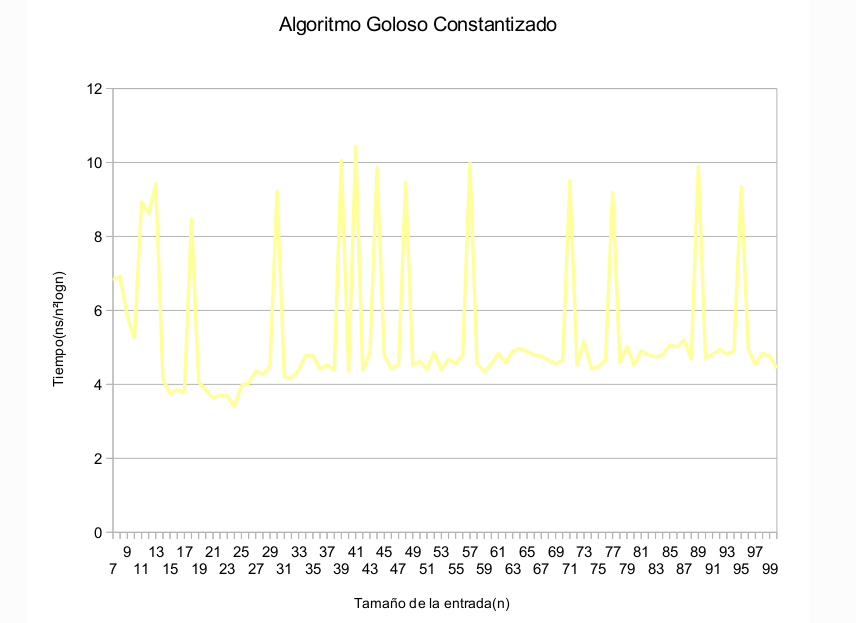
\includegraphics[width=1\textwidth]{goloso_grafico.png}

\subsubsection{Casos Patol�gicos}
Para la experimentacion de los casos patologicos, generamos un test que nos da grafos completos a los que a�adimos dos caminos, uno que 
miniza el peso $w_1$ 
y maximiza el peso $W_2$, y al revez para el otro. El hecho de que sean completos es por simplicidad en la implementacion. 
En el grafico presentamos la 
comparacion de los resultados contra el algoritmo exacto.

Podemos observar que los caminos difieren en la mayoria de los casos, y en los casos que no, se debe a que hay un camino dentro del subgrafo completo
de peso equivalente al optimo que agregamos.

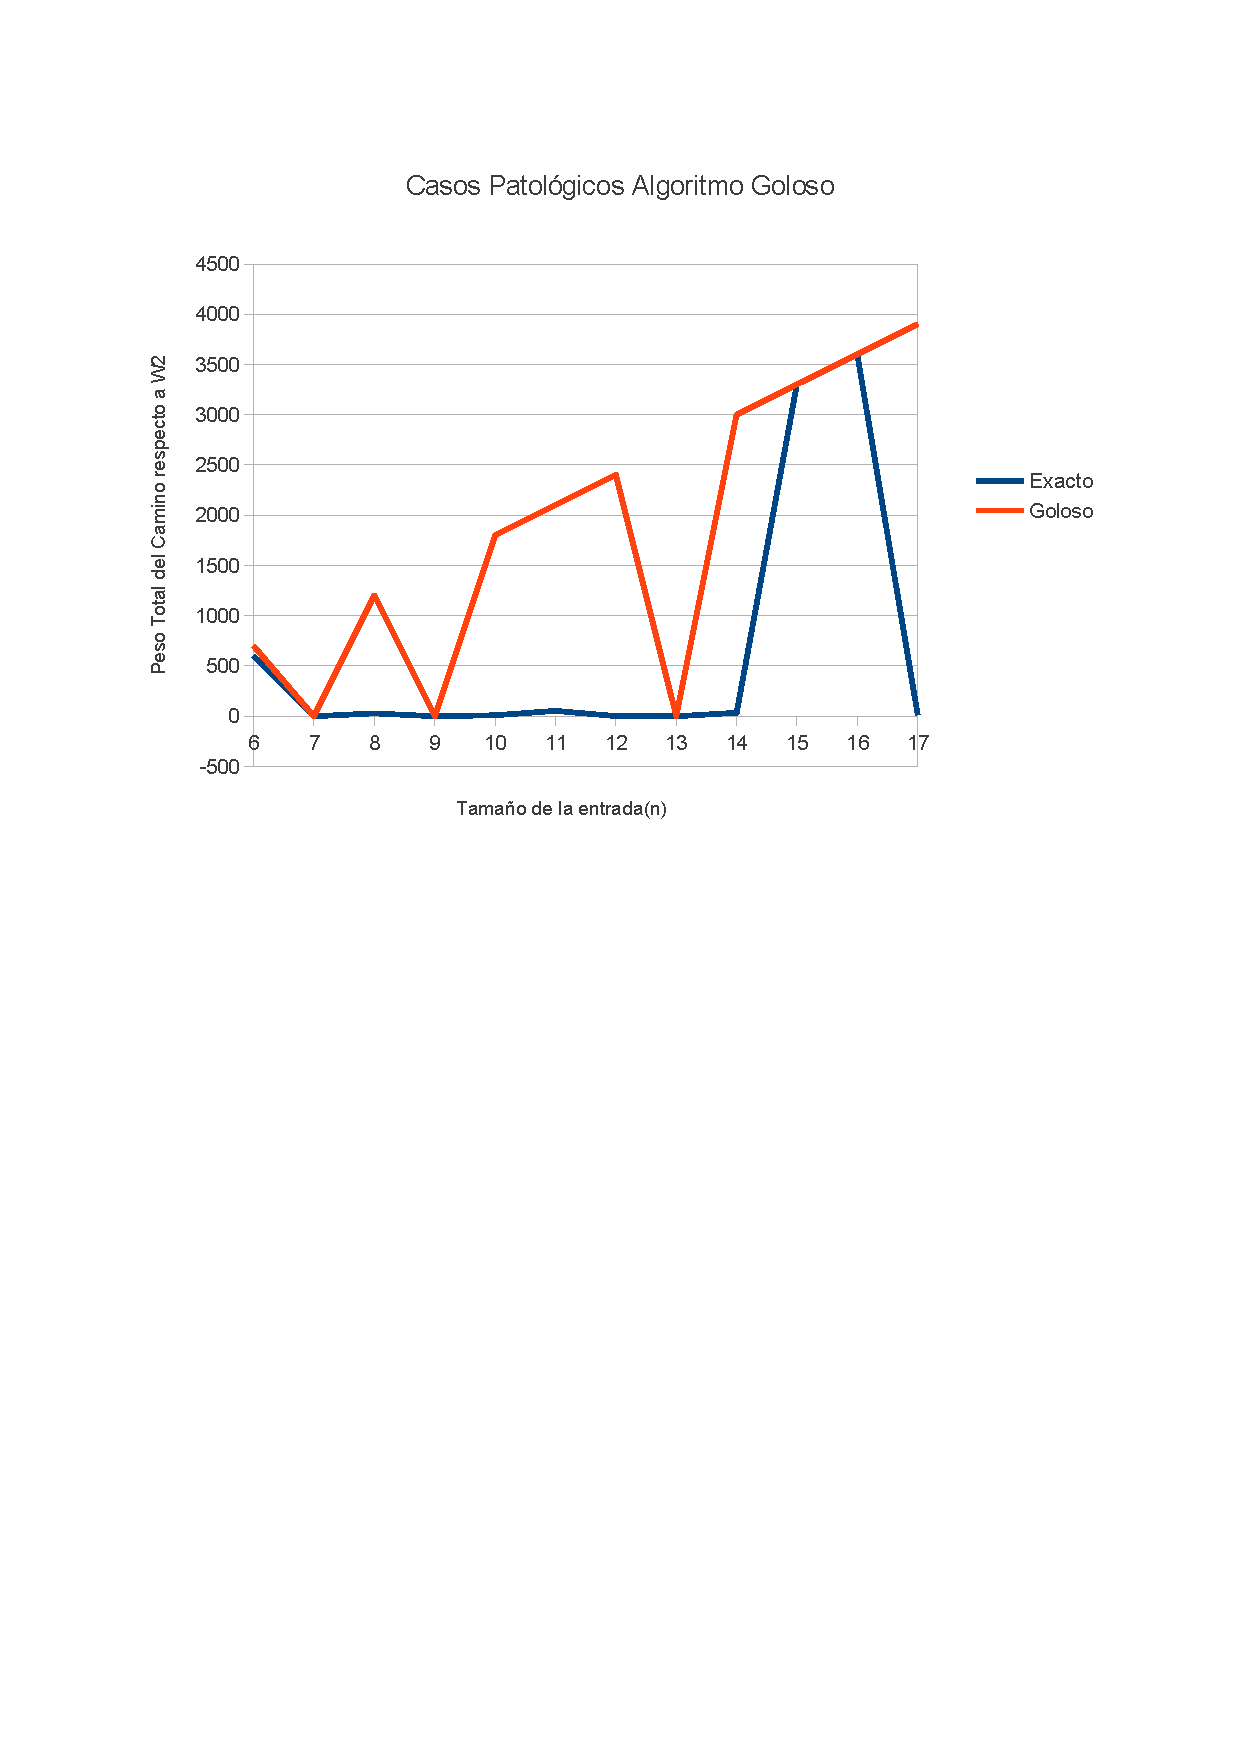
\includegraphics[width=1\textwidth]{casos_patologicos_goloso.pdf}